\documentclass[UTF8,nofonts]{ctexart}
\date{\today}
\usepackage{geometry}
\usepackage{fancyhdr}
\usepackage{amsmath}
\usepackage{algorithm2e}
\usepackage{graphicx}
\setCJKmainfont{微软雅黑}
\setmainfont{微软雅黑}
\linespread{1.6}
\geometry{a4paper,left=3cm,right=3cm,bottom=3cm}
\pagestyle{fancy}
\fancyhf{}
\rfoot{\thepage}
\lhead{ }
\renewcommand\headrulewidth{0.8pt}
\begin{document}
\newpage
\vspace{1cm}
\section{Principles of Neural Science:Memory}
在加西亚.马尔克斯的著名作品百年孤独中,描述了这样的一种奇怪的瘟疫。这个瘟疫袭击了一个小村庄,染上瘟疫的人会逐渐的丧失记忆:首先是个人的过往记忆,然后是常见器物的名字和用途。一个人为了与这种瘟疫做斗争,在自己家的所有器物上都贴上便笺。但是随着词语和字母的认知能力的丧失,一切抗争都归为徒劳。
\par
这段离奇故事从某个角度上说明了学习和记忆在我们日常生活中的作用。学习指的是通过获得的知识来改变行为,而记忆指的是我们对这些知识的编码、存储以及检索的过程。在1861年Broca发现左额叶的后部(Broca区)损伤会导致语言功能的退化,这个发现引发了脑功能区的划分热潮。脑功能区的离散划分自然而然的引发了下面这个问题:这些功能区是不是通过记忆相连的呢?如果真的是通过记忆相连的话,记忆是通过一个记忆中心相连呢还是广泛的分布于各脑区?
\par
过去的几十年中,学习和记忆方面的研究有了很大的进展。当前章节中,我们将注重于下面三个方面的介绍:
\begin{enumerate}
\item 学习和记忆有很多类型,不同的类型有不同的认知性质,由不同的脑区控制。
\item 记忆可以分解为编码、存储强化、检索这三个过程。
\item 记忆的相关异常可以为学习和记忆的研究提供线索。
\end{enumerate}
记忆能够分解为两个维度:时间维度和存储结构。我们这里首先来探讨一下时间维度。
\subsection{长期记忆和短期记忆牵涉到不同的神经系统}
\subsubsection{短期记忆维持当前目标相关信息的呈现}
当提到记忆的时候,我们一般想起的是长期记忆,而忽视了短期记忆。但是,长期记忆是由短期记忆固化而来的。短期记忆,也叫做\textit{working memory},维持着容易消失的当前目标相关知识的呈现。人类的\textit{work memory}至少包含两个子系统:一个与语言(verbal)相关,一个与视觉(visuospatial)相关。这两个子系统由第三个子系统--\textit{executive control process} 调控。这个\textit{executive control process} 的主要功能是分配注意力,监控、操控及更新所存储的知识表达。
\par
语言子系统又包括两个子系统:一个用来存储语音相关的知识,一个用来回响接收的语音输入。神经生理学和神经成像的数据表明:语音知识的存储与后顶叶皮层有关,而回响则需要Broca区的参与。
\par
视觉子系统又与顶叶、内测颞叶、枕骨外皮层、前额叶、运动前皮层相关。至于这个视觉子系统是否可以分解为空间和物体这两个子系统,人们目前还没有定论。
\subsubsection{短期记忆会被选择性的转换为长期记忆}
在1950年代,学界从癫痫病人的切除治疗中获得了长期记忆是从短期记忆转换而来的惊人证据。这些病人的中颞叶的双侧海马和附近区域都被切除了,由此造成了这些病人的长期记忆形成障碍。这些病人中,最出名的就是代号为H.M.(为了维护病人隐私)的病人,心理学家Brenda Milner和外科医师William Scoville对这个病人做了长期的观察。2008-12-1,H.M.去世,他的真实姓名Henry Molaison才被披露出来。
\par
当时,病人H.M.为27岁的男性,7岁时由于自行车事故引起了脑部损伤,并因此忍受了10多年的不可治疗的颞叶癫痫。Scoville移除了这个病人的海马组织、杏仁核和双侧颞叶的multimodal association 区。在这个手术之后,H.M.的癫痫得到了很好的控制,但是他的记忆却损伤很大。但是,HM的记忆损伤非常特别,这种情况引起了人们的注意。
\par
HM仍然有正常的短期记忆(working memory),从几秒到几分钟不等。这个症状说明,中颞叶对于短期记忆来说并不是必须的。此外,HM对于手术之前的长期记忆仍然保持的很好。HM现在最主要的记忆困难是无法将新的短期记忆转换为长期记忆。他无法在记忆中维持刚刚认识的人、刚刚经历过的事情这些信息。当被要求背诵一个电话号码的时候,HM在几分钟之内仍然能够很好的完成这项任务。但是一旦将他的注意力转移,HM则会丧失对这个电话号码的记忆。HM并不是一个孤立的现象,所有经历过广泛双侧中间颞叶切除的病人都或多或少的会有短期记忆无法转换到长期记忆的症状。
\par
HM的重要性在于,他的功能损伤是证明记忆与中间颞叶(包括海马体)有关的第一个有效证据。考虑到海马体的大小比较大,人们不禁想知道:到底多大的损伤才会导致长期记忆困难?另外一个病人RB的临床病例表明,即使海马体只受损了一小部分,长期记忆仍然会受到很大的损伤。不同部位的损伤造成的后果可能不一样,例如海马体下面的前内鼻区(perirhinal)皮层损伤对于物体识别的影响比海马体上面的皮层损伤所造成的影响大。一些学者认为,海马体在空间认知方面的重要性比物体识别的重要性大得多。在人类身上的脑功能成像实验表明:右侧海马在涉及到空间信息记忆的行为中活动增强,而左侧海马在涉及到文字、物体及人物识别行为中活动增强。这个结论与临床上相关区域受损病人的症状相吻合。
\subsubsection{长期记忆可以分为显式记忆和隐式记忆}
在病人HM身上还观察到另外一个症状:并不是所有类型的长期记忆都完全受损,有些类型的长期记忆甚至是完全正常的。经历过类似手术病人大多也有这种症状。这种未受损的长期记忆大都来自于反射学习:即长期的重复某些活动从而得到了这个活动的长期记忆。比较生动形象的例子就是学自行车。但是反射学习并不仅仅限制在运动学习这一块,还包括habituation ,sensitization ,classical conditioning and operant conditioning。这类反射学习相关的记忆叫做隐式记忆(nondeclarative or procedural memory),这类记忆的检索完完全全是在意识无关的状态下进行的。而另外一种需要在意识作用下检索的记忆叫做显式记忆(declarative memory),它主要包括对于人、物和地点的事实知识。显式记忆是非常灵活的,多种不同环境的记忆片段可以一起链接起来。而隐式记忆则限制在特定场景下才能触发,也就是当时学习的环境条件。
\subsubsection{显式记忆拥有片段及语义形式}
加拿大心理学家Endel Tulving第一次提出了下面的观点:显示记忆可以被分类为两类-片段记忆(episodic memory)和语义(semantic)记忆。场景记忆是用来存储个人经历相关的知识,而语义记忆则是用来存储词汇和概念的意义。
\begin{figure}[h]
\centering
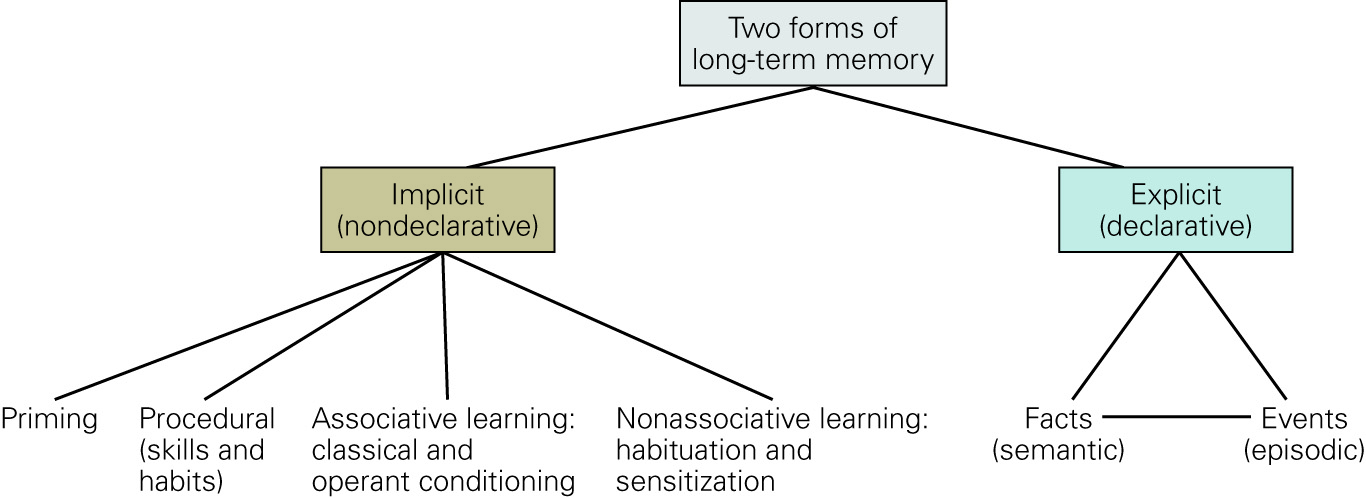
\includegraphics{Pic/6505_PNS5.jpg}
\end{figure}
对于显式记忆,我们还有如下的认识。
\begin{enumerate}
\item 大脑并没有一个单一的长期的显式记忆存储,而是分布在大脑的各个部分。这些不同部分的记忆检索可以被不同的方式独立触发,例如视觉、语音以及其他的感官信息。
\item 显式记忆至少有四个不同的信息处理过程: 编码(encoding),存储(storage),强化(consolidation),检索(retrieval)。这里我就不详细说了。
\end{enumerate}
\subsubsection{场景记忆依赖于中颞叶与相关皮层的交互}
临床失忆症病例表明,中颞叶的受损会影响在记忆上的所有四种操作:编码,存储,强化,检索,很难按照区域对功能进行定位。在PET和fMRI的帮助下,我们才能具体的观察各个不同区域在不同操作下的影响。fMRI表明:在涉及到深度编码(例如判断一个单词是具体还是抽象)时中颞叶的活动比浅显编码(例如是否一个单词是大写的还是小写的)时活动更强。左前额叶皮层在深度编码时,活动也会增强。这些证据表明前额叶与中颞叶在编码场景记忆是有很大的作用。后续的实验表明:场景记忆依赖于前额叶的认知控制过程和中颞叶的关联绑定机制之间的交互。
\par
中颞叶的不同的皮质区之间的交互对于记忆强化这个过程非常重要。HM的事例表明,老的记忆并不存储在中颞叶这里。根据Larry Squire等人的相关研究,中颞叶在记忆强化过程中只是当作一个临时存储区,这个存储区所存储的记忆会随着时间而衰退,而这些衰退的记忆会转移到皮质区。当记忆检索的时候,会同时检索这两个区域。失忆病人的症状与这个推论相吻合。
\par

\end{document}